\documentclass[tikz,border=5pt]{standalone}
\usepackage[T1]{fontenc}
\usepackage{lmodern,amsmath,amssymb}
\usetikzlibrary{arrows.meta,calc,positioning,fit,backgrounds,shapes.geometric,matrix,decorations.pathreplacing,patterns}
\definecolor{ink}{gray}{0.08}
\definecolor{wash}{gray}{0.965}
\definecolor{soft}{gray}{0.45}
\tikzset{box/.style={draw=ink,line width=.65pt,fill=white,align=center,inner sep=4pt,outer sep=0pt,font=\small},flow/.style={draw=ink,line width=.65pt,-{Latex[length=1.8mm,width=1.3mm]},rounded corners=2pt},annotation/.style={font=\scriptsize,text=soft,align=center},groupbox/.style={draw=soft,dashed,line width=.45pt,fill=wash}}
\begin{document}
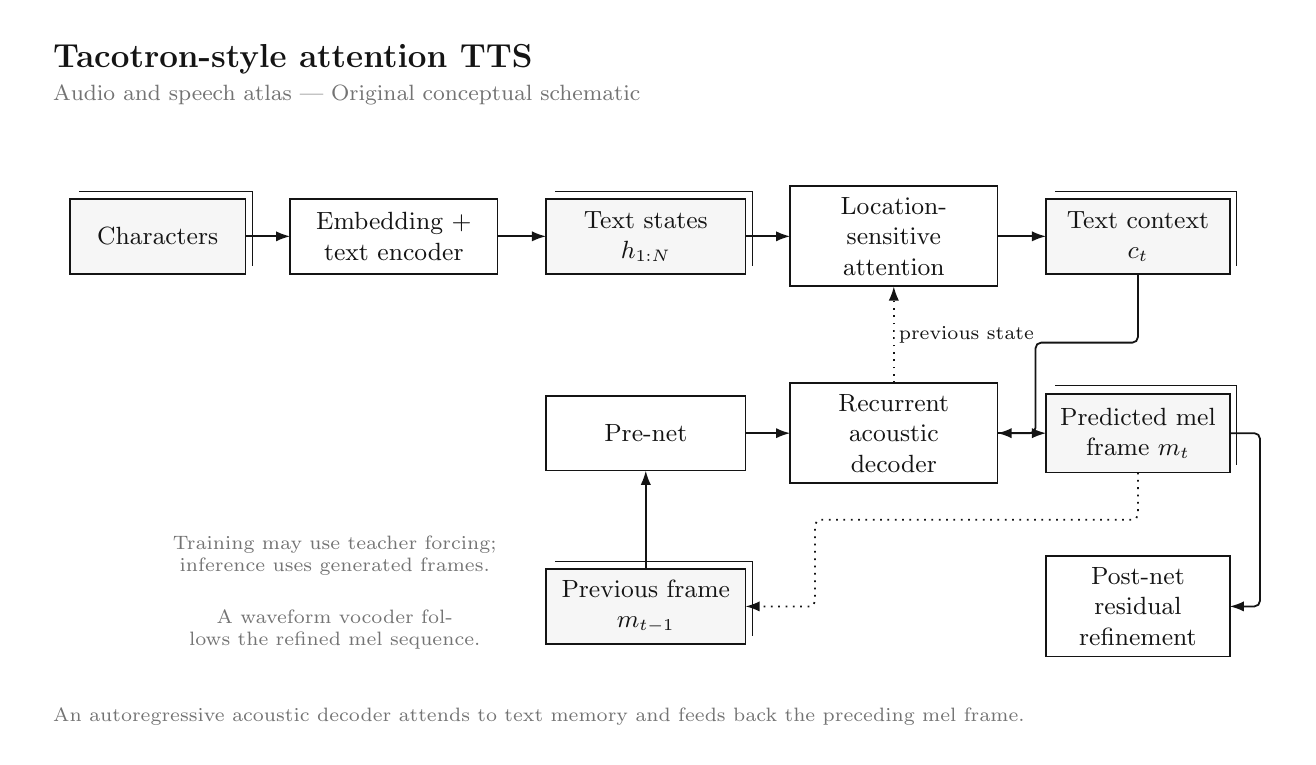
\begin{tikzpicture}[x=1cm,y=-1cm,font=\rmfamily,text=ink]

\path[use as bounding box] (0,0) rectangle (16,9);
\node[anchor=west,font=\large\bfseries] at (.2,.4) {Tacotron-style attention TTS};
\node[anchor=west,font=\footnotesize,text=soft] at (.2,.85) {Audio and speech atlas | Original conceptual schematic};
\begin{pgfonlayer}{background}
\end{pgfonlayer}
\node[box,fill=wash,minimum width=2.2cm,minimum height=0.95cm,text width=1.9500000000000002cm] (text) at (1.65,2.65) {Characters};
\draw[ink,line width=.4pt] (0.6499999999999998,2.0749999999999997) -- (2.85,2.0749999999999997) -- (2.85,3.025);
\node[box,minimum width=2.6cm,minimum height=0.95cm,text width=2.35cm] (encoder) at (4.65,2.65) {Embedding +\\text encoder};
\node[box,fill=wash,minimum width=2.5cm,minimum height=0.95cm,text width=2.25cm] (memory) at (7.85,2.65) {Text states\\$h_{1:N}$};
\draw[ink,line width=.4pt] (6.699999999999999,2.0749999999999997) -- (9.2,2.0749999999999997) -- (9.2,3.025);
\node[box,minimum width=2.6cm,minimum height=0.95cm,text width=2.35cm] (attn) at (11.0,2.65) {Location-sensitive\\attention};
\node[box,fill=wash,minimum width=2.3cm,minimum height=0.95cm,text width=2.05cm] (context) at (14.1,2.65) {Text context\\$c_t$};
\draw[ink,line width=.4pt] (13.049999999999999,2.0749999999999997) -- (15.35,2.0749999999999997) -- (15.35,3.025);
\node[box,minimum width=2.5cm,minimum height=0.95cm,text width=2.25cm] (prenet) at (7.85,5.15) {Pre-net};
\node[box,minimum width=2.6cm,minimum height=1.0cm,text width=2.35cm] (decoder) at (11.0,5.15) {Recurrent acoustic\\decoder};
\node[box,fill=wash,minimum width=2.3cm,minimum height=1.0cm,text width=2.05cm] (mel) at (14.1,5.15) {Predicted mel\\frame $m_t$};
\draw[ink,line width=.4pt] (13.049999999999999,4.550000000000001) -- (15.35,4.550000000000001) -- (15.35,5.550000000000001);
\node[box,fill=wash,minimum width=2.5cm,minimum height=0.95cm,text width=2.25cm] (previous) at (7.85,7.35) {Previous frame\\$m_{t-1}$};
\draw[ink,line width=.4pt] (6.699999999999999,6.775) -- (9.2,6.775) -- (9.2,7.725);
\node[box,minimum width=2.3cm,minimum height=0.95cm,text width=2.05cm] (post) at (14.1,7.35) {Post-net residual\\refinement};
\begin{pgfonlayer}{background}
\draw[flow] (text.east) -- (encoder.west);
\draw[flow] (encoder.east) -- (memory.west);
\draw[flow] (memory.east) -- (attn.west);
\draw[flow] (attn.east) -- (context.west);
\draw[flow] (previous.north) -- (prenet.south);
\draw[flow] (prenet.east) -- (decoder.west);
\draw[flow] (decoder.east) -- (mel.west);
\draw[flow,dotted] (decoder.north) -- (attn.south) node[midway,right,fill=white,inner sep=1.5pt,font=\scriptsize] {previous state};
\draw[flow] (context.south) -- (14.1,4.0) -- (12.8,4.0) -- (12.8,5.15) -- (decoder.east);
\draw[flow,dotted] (mel.south) -- (14.1,6.25) -- (10.0,6.25) -- (10.0,7.35) -- (previous.east);
\draw[flow] (mel.east) -- (15.65,5.15) -- (15.65,7.35) -- (post.east);
\end{pgfonlayer}
\node[align=center,anchor=center,font=\scriptsize,text=soft,text width=6.6cm] at (3.9,6.7) {Training may use teacher forcing; inference uses generated frames.};
\node[align=center,anchor=center,font=\scriptsize,text=soft,text width=6.6cm] at (3.9,7.65) {A waveform vocoder follows the refined mel sequence.};
\node[anchor=west,align=left,font=\scriptsize,text=soft,text width=15.6cm] at (.2,8.75) {An autoregressive acoustic decoder attends to text memory and feeds back the preceding mel frame.};
\end{tikzpicture}
\end{document}
